\documentclass{article}
\usepackage[utf8]{inputenc}
\usepackage{graphicx}
\usepackage{titling}
\usepackage{amsmath}
\usepackage{amssymb}
\usepackage{cite}
\usepackage{hyperref}
\usepackage{float}
\usepackage{listings}
\usepackage{xcolor}
\usepackage{geometry}
\geometry{a4paper, margin=1in}


\begin{document}

\definecolor{codegreen}{rgb}{0,0.6,0}
\definecolor{codegray}{rgb}{0.5,0.5,0.5}
\definecolor{codepurple}{rgb}{0.58,0,0.82}
\definecolor{backcolour}{rgb}{0.95,0.95,0.92}

\lstdefinestyle{pythonstyle}{
    backgroundcolor=\color{backcolour},   
    commentstyle=\color{codegreen},
    keywordstyle=\color{magenta},
    numberstyle=\tiny\color{codegray},
    stringstyle=\color{codepurple},
    basicstyle=\ttfamily\footnotesize,
    breakatwhitespace=false,         
    breaklines=true,                 
    captionpos=b,                    
    keepspaces=true,                 
    numbers=left,                    
    numbersep=5pt,                  
    showspaces=false,                
    showstringspaces=false,
    showtabs=false,                  
    tabsize=2
}

\lstset{style=pythonstyle}




% Custom title page
\begin{titlepage}
    \begin{center}
        \begin{minipage}[c]{0.12\textwidth}
            
\includegraphics[width=\textwidth]{Cairo_University_Crest.png}
        \end{minipage}
        \hfill
        \begin{minipage}[c]{0.5\textwidth}
            \centering
            {\large Cairo University - Faculty Of Engineering \\ Computer Engineering Department \\ Digital Communication  - Spring 2025 \par}
        \end{minipage}
        \hfill
        \begin{minipage}[c]{0.15\textwidth}
            
\includegraphics[width=\textwidth]{CUFE.jpeg}
        \end{minipage}
    \end{center}
    
    \noindent\hrulefill
    
    \vspace{2cm}
    
    \begin{center}
        {\Huge \textbf{Digital Communications: Assignment 1 (Quantization)}\par}
        \vspace{1.5cm}

        {\large Submitted to\par}
        {\Large \textbf{Dr. Mai Badawi }\par}
        {\Large \textbf{Dr. Hala }\par}
        {\Large \textbf{Eng. Mohamed Khaled }\par}
        \vspace{1cm}
        
        {\large Submitted by\par}
        {\Large \textbf{Akram Hany Sec 1 BN 14 }\par}
        {\Large \textbf{Amir Anwar Sec 1 BN 15 }\par}
        \vspace{1cm}
        
    \end{center}
    
    \vfill
    
\end{titlepage}

% Add Table of Contents
\tableofcontents
\newpage

% Add List of Figures
\listoffigures
\newpage

\section{Introduction}

In this report, we provide our solution / implementation for Quantization. Covering concepts like midtread and midrise, SNR, uniform and non-uniform quantizers.

\section{General Theoretical Background}

\subsection{Uniform Quantization}

\begin{itemize}
    \item Number of levels: $L = 2^n$ where $n$ is the number of bits
    \item Level amplitude: $\Delta = \frac{A_{max} - A_{min}}{L}$
    \item Quantization error: $q = \frac{\Delta}{2}$
\end{itemize}

The quantization error is bounded by: $-\frac{\Delta}{2} < q \leq \frac{\Delta}{2}$

\subsection{Signal-to-Noise Ratio (SNR)}

For uniform quantization, the theoretical SNR can be calculated as:

$$SNR_{avg} = \frac{3\alpha L^2}{\Delta^2/12} = 3\alpha 2^{2n}$$

Where $\alpha$ is a signal-dependent parameter. In decibels:

$$SNR_{Peak} = 10\log_{10}(3\alpha) + 6n$$


\subsection{Midtread and Midrise Quantizers}

The types of uniform quantizers are midtread and midrise:

\begin{itemize}
    \item \textbf{Midtread Quantizer}: voltage levels includes zero
    \item \textbf{Midrise Quantizer}: voltage levels doesn't include a level at zero
\end{itemize}

\subsection{Non-uniform Quantization}

For non-uniform signals in uniform quantizers, the SNR performance degrades. To improve performance, non-uniform quantization through using a compressor and an expander can be used, the SQNR given by:

$$SQNR_{non-uniform} = \frac{3L^2}{\ln^2(1+\mu)}$$

Where $\mu$ is the compression parameter.

\section{Results and comments}

\subsection{Midtread and Midrise Quantization (part 1,2,3)}

\begin{figure}[H]
    \centering
    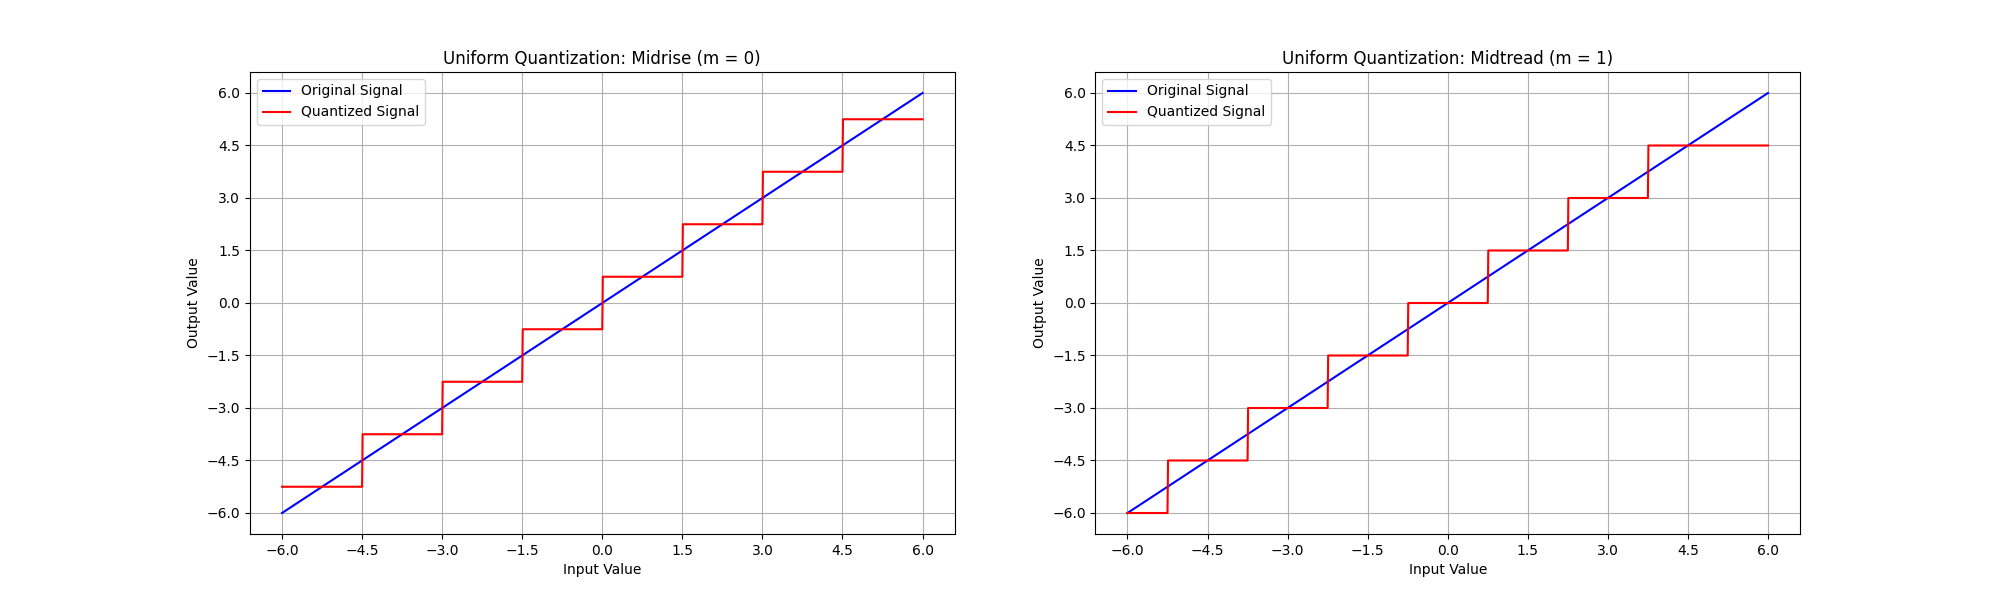
\includegraphics[width=1\textwidth]{quantization_comparison.png}
    \caption{Original (input) signal and its dequantized version using midtread (m=1) and midrise (m=0)}
    \label{fig:midtread_midrise}
\end{figure}


Figure \ref{fig:midtread_midrise} shows the original signal and its quantized version for both midtread (m=1) and midrise (m=0) quantizers. The midtread quantizer includes a level at zero, while the midrise quantizer has levels at half-integer values.

\textbf{Note:} We adjusted the lower bound clipping in the quantizer implementation to allow the -6 level to appear in the output, which causes the quantization to appear asymmetric (showing 7 levels instead of the expected 8 levels). This adjustment was made to better demonstrate the behavior of the quantizer at the signal extremes. And to match our tutorial quantizer graphs.

\begin{figure}[H]
    \centering
    \includegraphics[width=1\textwidth]{tutorial.png}
    \caption{Tutorial midrise and midtread demonostration graph}
    \label{fig:tutorial}
\end{figure}


\begin{figure}[H]
    \centering
    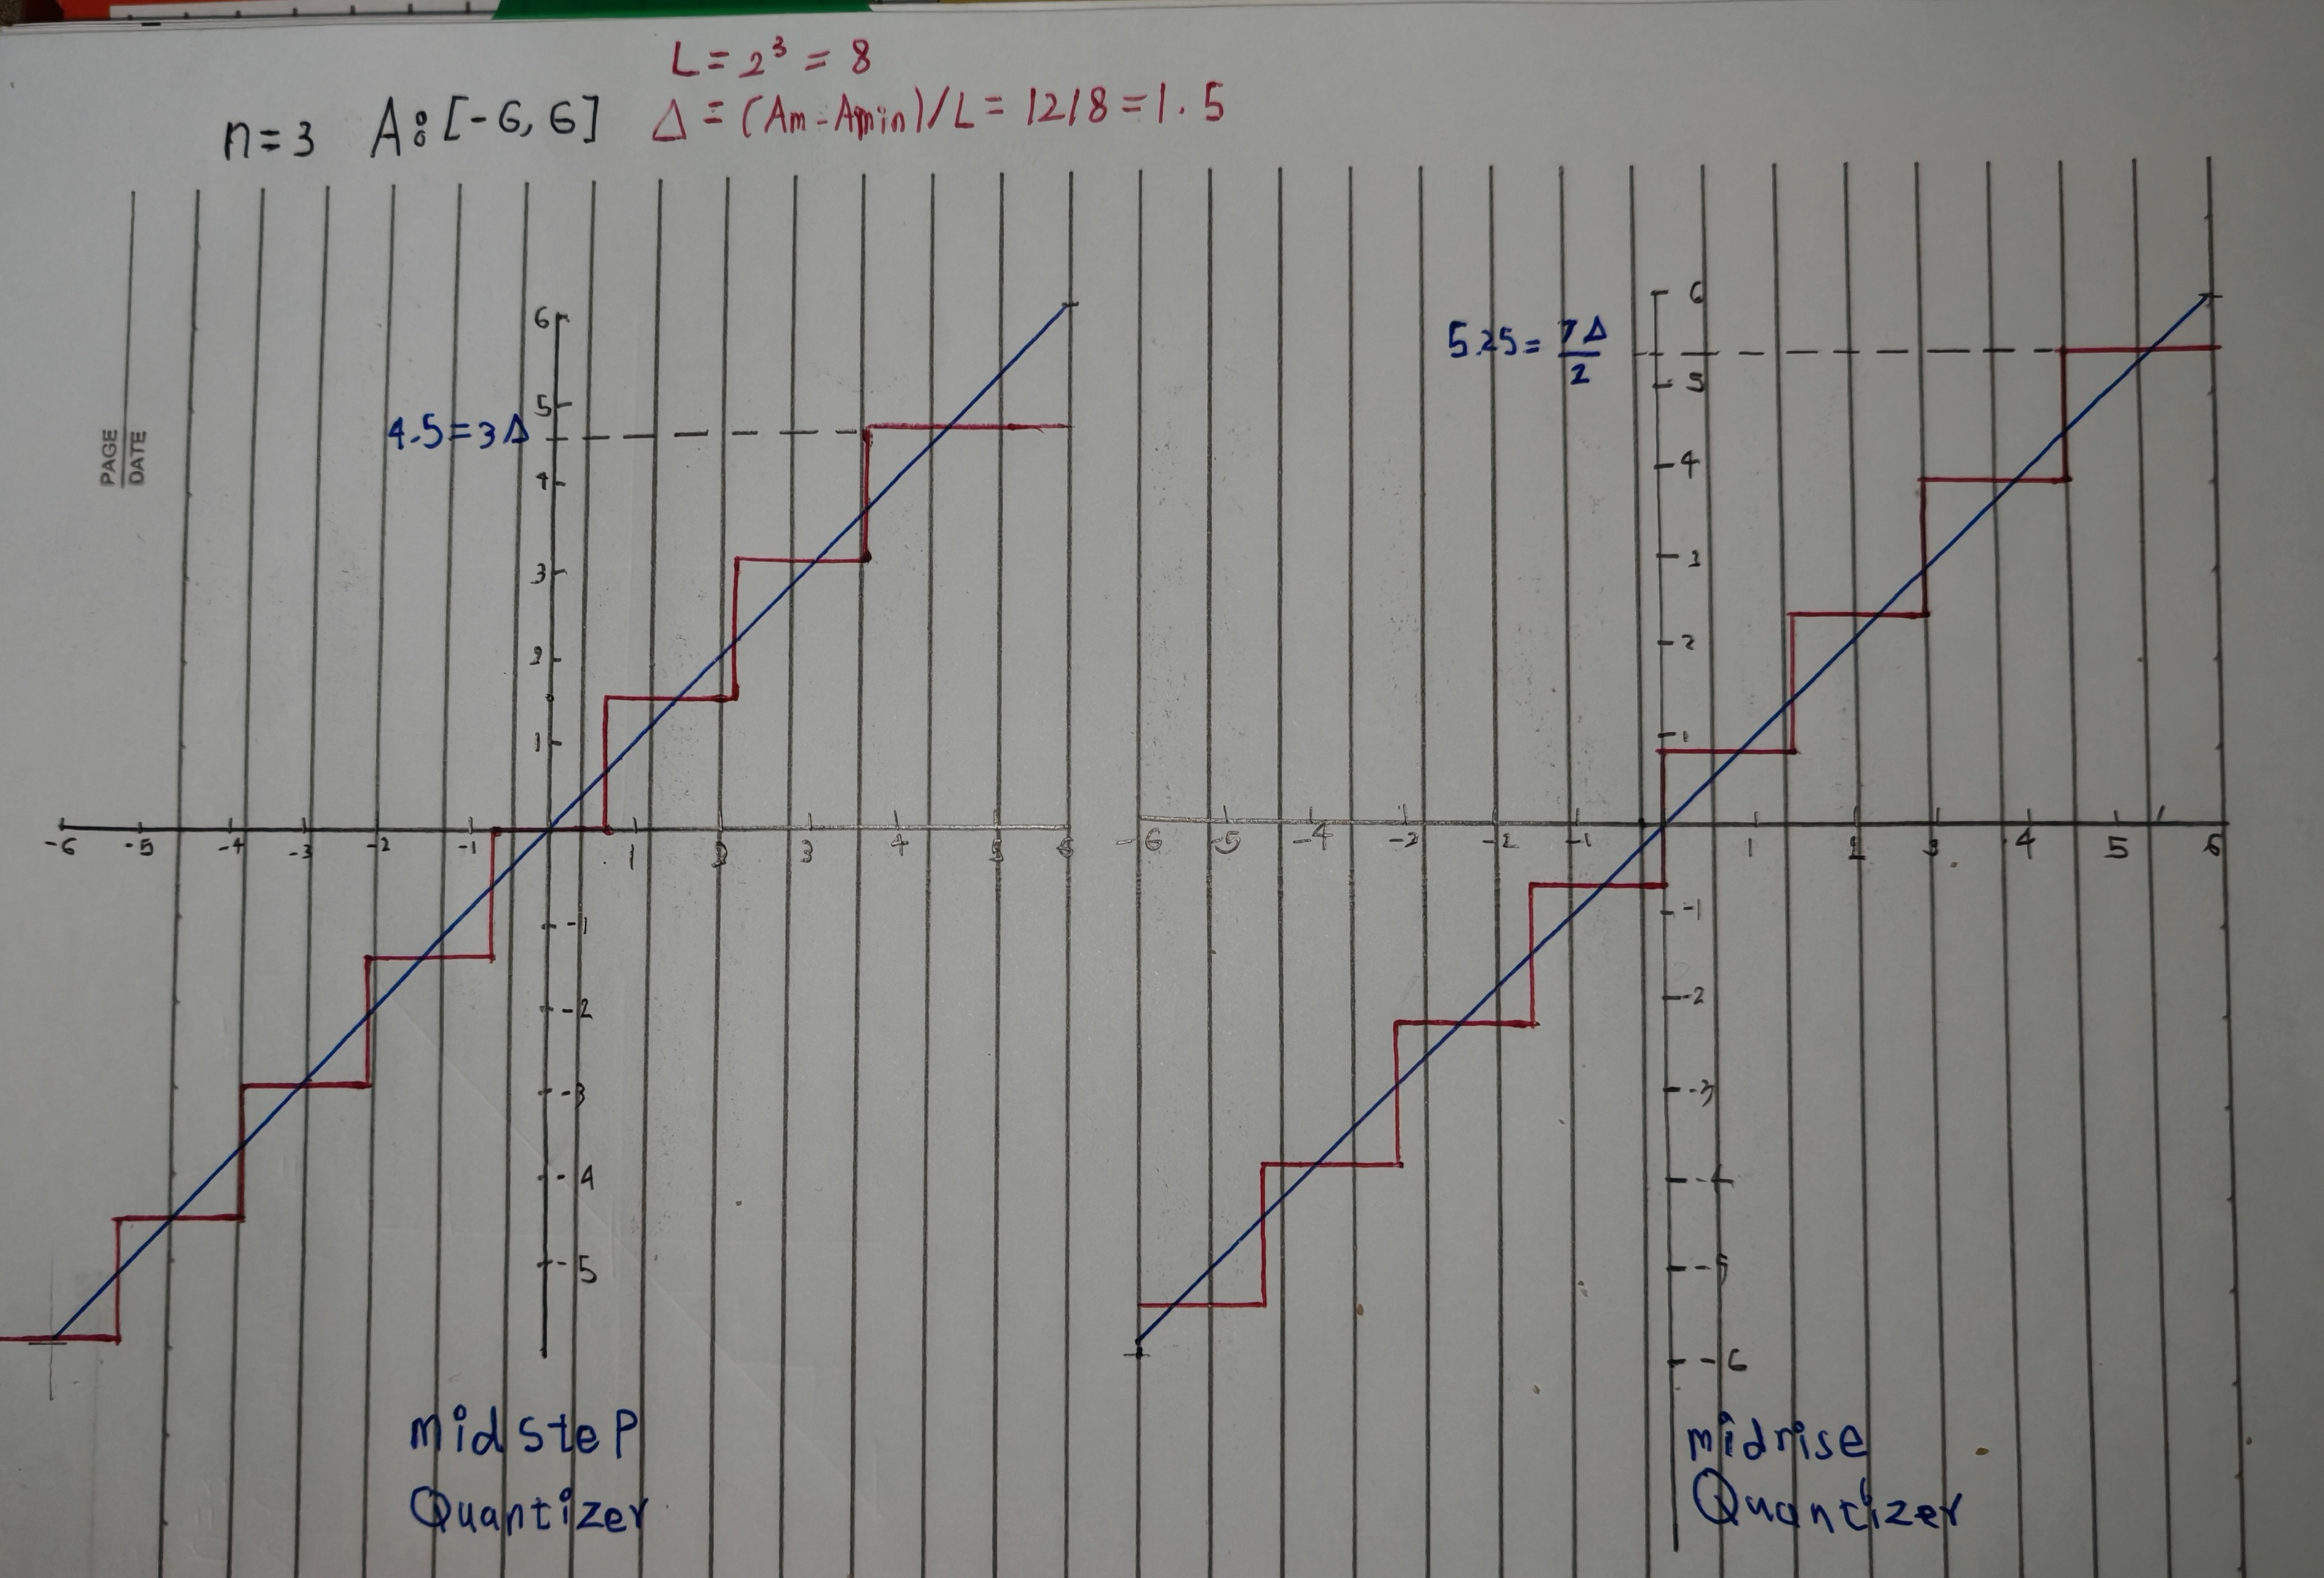
\includegraphics[width=1\textwidth]{figure-2.jpg}
    \caption{Manual calculation and hand-drawing of quantization processes for verification}
    \label{fig:manual_calc}
\end{figure}

Figure \ref{fig:manual_calc} presents a manual calculation and hand-drawing of the same quantization processes to verify the results. Showing on the 2 graphs:

\begin{enumerate}
    \item{the signal maximum value for both}
    \item{midtrade have a level at 0 while midrise doesn't}
    \item{midrise have equal number of levels above and under 0}
    \item{midtrade levels are integer multiple of $\Delta$}
    \item{midrise step (input level boundaries) are integer multiple of $\Delta$}
\end{enumerate}

\textbf{Note:} All equations for this part are in the \textit{General Theoretical Background} Section.


\subsection{SNR Analysis for uniform signal (part 4)}

\begin{figure}[H]
    \centering
    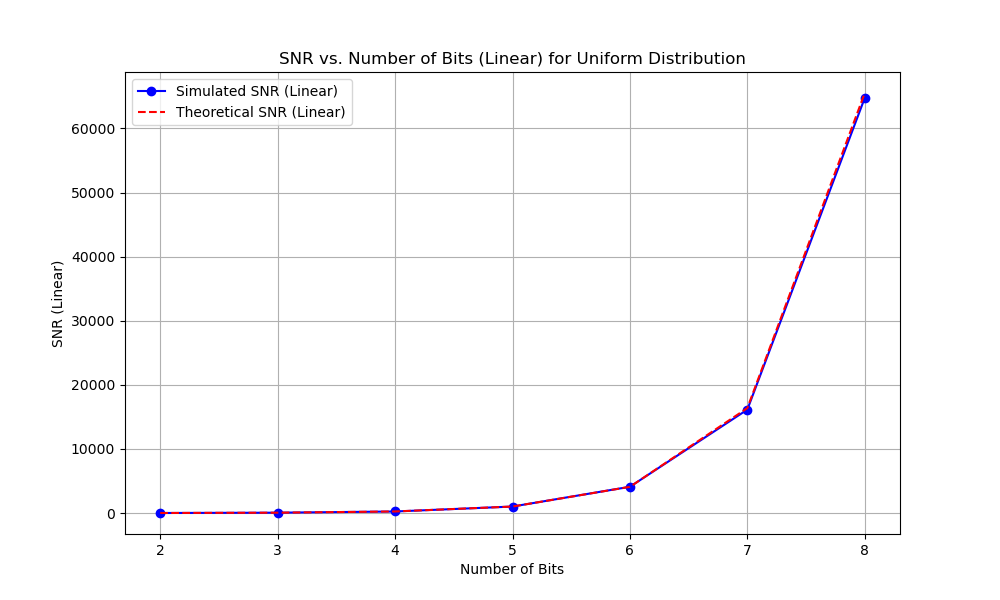
\includegraphics[width=1\textwidth]{uniform_snr_linear.png}
    \caption{SNR across different bit depths (n) - Linear scale}
    \label{fig:snr_linear}
\end{figure}

Figure \ref{fig:snr_linear} displays the SNR across different bit depths (n) for both theoretical and calculated values in linear scale. As expected, the SNR increases linearly with the number of bits.

\begin{figure}[H]
    \centering
    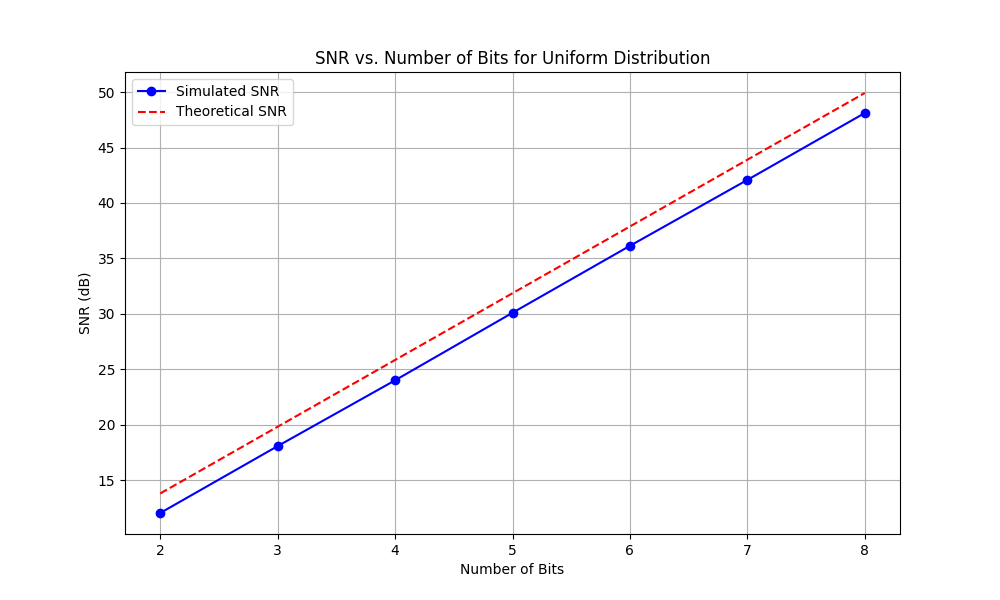
\includegraphics[width=1\textwidth]{uniform_snr.png}
    \caption{SNR across different bit depths (n) - Decibel scale}
    \label{fig:snr_db}
\end{figure}

Figure \ref{fig:snr_db} presents the same data in decibel scale, showing the expected 6 dB improvement in SNR for each additional bit of quantization.  Additionaly because we have a uniform signal the Simulated/calculated SNR almost matches with the theoretical SNR.

\subsection{SNR Analysis for nonuniform signal (part 5)}

\begin{figure}[H]
    \centering
    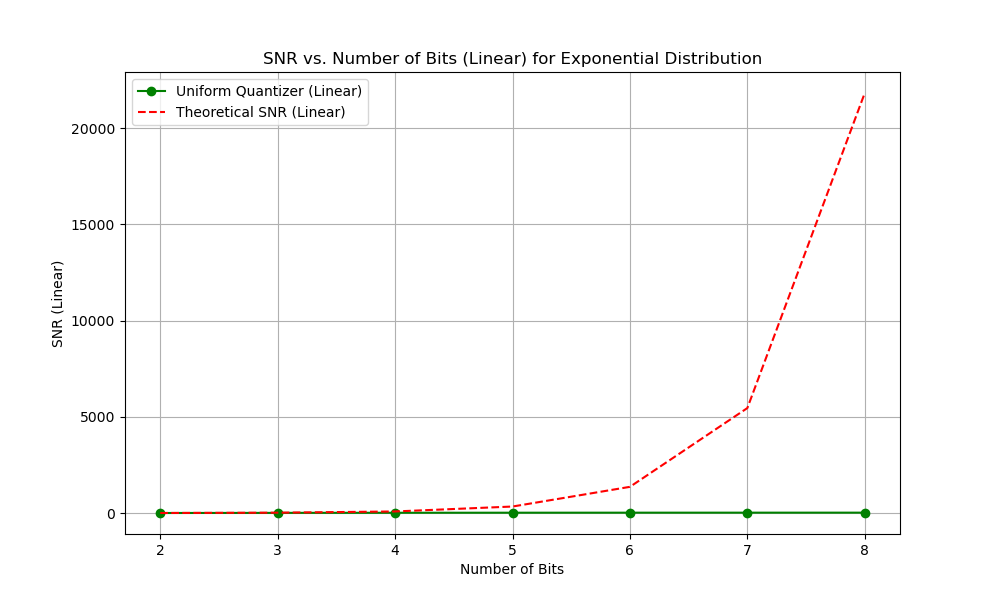
\includegraphics[width=1\textwidth]{nonuniform_snr_linear.png}
    \caption{SNR for non-uniform signals in uniform quantizers - Linear scale}
    \label{fig:nonuniform_linear}
\end{figure}

\begin{figure}[H]
    \centering
    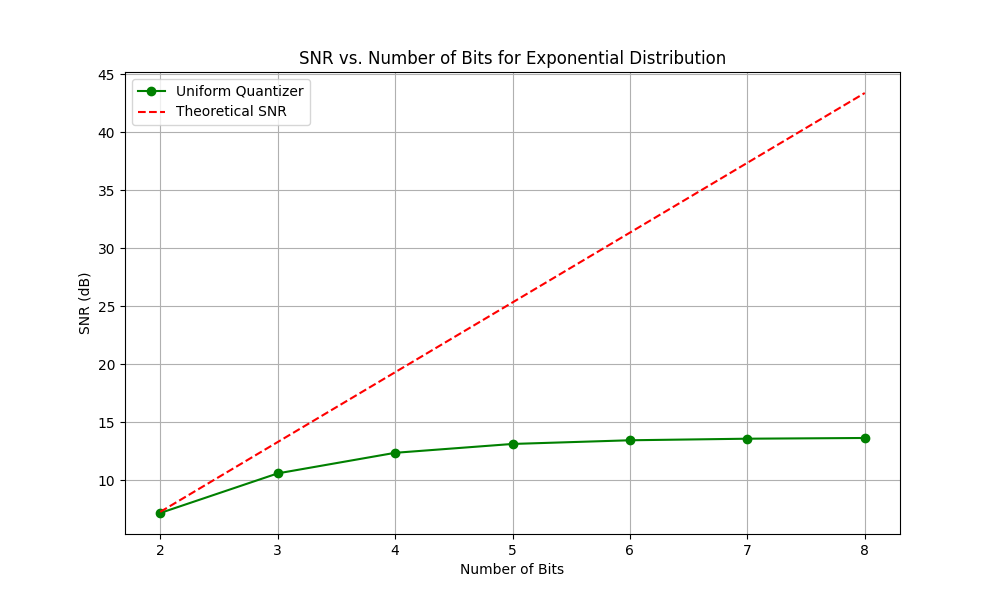
\includegraphics[width=1\textwidth]{nonuniform_snr.png}
    \caption{SNR for non-uniform signals in uniform quantizers - Decibel scale}
    \label{fig:nonuniform_db}
\end{figure}

Figures \ref{fig:nonuniform_linear} and \ref{fig:nonuniform_db} show the SNR performance for non-uniform signals processed through uniform quantizers, highlighting the degradation in performance compared to uniform signals.

\vspace{0.5cm}

This happens because the signal is not equally distributed between the levels like in uniform signals (for example all signals most of the signals should be centered in one level increasing the error significantly). Even though this happens uniform quantizer could still be used using compressor and expander before and after the quantization and dequantization.


\subsection{Compressor Expander to use uniform quantizer with nonuniform signals}

\begin{figure}[H]
    \centering
    \includegraphics[width=0.8\textwidth]{tutorial-2.png}
    \caption{Compressor Quantizer Expander block diagram}
    \label{fig:tutorial-compressor}
\end{figure}

\begin{figure}[H]
    \centering
    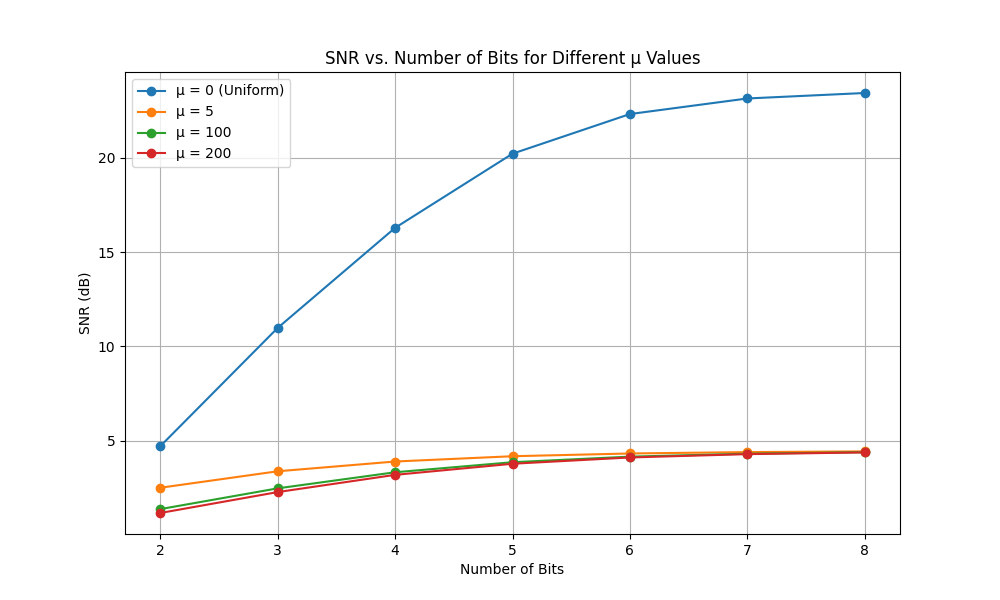
\includegraphics[width=1\textwidth]{mu_law_comparison.png}
    \caption{Effect of compression parameter ($\mu$) on SNR performance}
    \label{fig:expander}
\end{figure}

Figure \ref{fig:expander} illustrates the effect of different compression parameters ($\mu$) on the SNR performance of the compander-expander system. Appropriate selection of $\mu$ can optimize performance for specific signal distributions.

\section{Conclusion}

Our analysis confirms the theoretical expectations regarding quantization performance:

\begin{enumerate}
    \item The SNR improves by approximately 6 dB for each additional bit in the quantizer
    \item Midtread and midrise quantizers show different characteristics, particularly in how they handle signals near zero
    \item Non-uniform signals experience degraded performance in uniform quantizers
    \item using (compressing and expanding) can significantly improve performance for non-uniform signals when the compression parameter is properly selected
\end{enumerate}

\appendix

\section{Python Implementation}
\subsection{Quantizer and Dequantizer Implementation}

\begin{lstlisting}[language=Python, caption=Uniform Quantizer and Dequantizer Functions]
import numpy as np

def uniform_quantizer(in_val, n_bits, xmax, m):
    L = 2 ** n_bits
    delta = (2 * xmax) / L
    
    lower_bound = -xmax
    higher_bound = m * delta / 2 + xmax
    
    in_val_clipped = np.clip(in_val, lower_bound, higher_bound)
    q_ind = np.floor((in_val_clipped + (m * delta / 2) + xmax) / delta)
    q_ind = np.clip(q_ind, 0, L - 1).astype(int)
    
    return q_ind

def uniform_dequantizer(q_ind, n_bits, xmax, m):
    L = 2 ** n_bits
    delta = (2 * xmax) / L
    
    deq_val = (q_ind * delta) - xmax + ((1 - m) * delta / 2)
    
    return deq_val
\end{lstlisting}

\subsection{Midtread and Midrise Visualization}

\begin{lstlisting}[language=Python, caption=Midtread and Midrise Quantization Visualization]
def plot_midtread_midrise_comparison():
    x = np.arange(-6, 6.01, 0.01)
    n_bits = 3
    xmax = 6

    # Test for m = 0 (midrise)
    m = 0
    q_ind = uniform_quantizer(x, n_bits, xmax, m)
    y_midrise = uniform_dequantizer(q_ind, n_bits, xmax, m)

    # Test for m = 1 (midtread)
    m = 1
    q_ind = uniform_quantizer(x, n_bits, xmax, m)
    y_midtread = uniform_dequantizer(q_ind, n_bits, xmax, m)

    plt.figure(figsize=(20, 6))

    plt.subplot(1, 2, 1)
    plt.plot(x, x, "b-", linewidth=1.5, label="Original Signal")
    plt.plot(x, y_midrise, "r-", linewidth=1.5, label="Quantized Signal")
    plt.title("Uniform Quantization: Midrise (m = 0)")
    plt.xlabel("Input Value")
    plt.ylabel("Output Value")
    plt.legend()
    plt.grid(True)
    plt.xticks(np.arange(-6, 7, 1.5))
    plt.yticks(np.arange(-6, 7, 1.5))

    plt.subplot(1, 2, 2)
    plt.plot(x, x, "b-", linewidth=1.5, label="Original Signal")
    plt.plot(x, y_midtread, "r-", linewidth=1.5, label="Quantized Signal")
    plt.title("Uniform Quantization: Midtread (m = 1)")
    plt.xlabel("Input Value")
    plt.ylabel("Output Value")
    plt.legend()
    plt.grid(True)
    plt.xticks(np.arange(-6, 7, 1.5))
    plt.yticks(np.arange(-6, 7, 1.5))

    plt.savefig("quantization_comparison.png")
    plt.show()
\end{lstlisting}

\subsection{Uniform Signal SNR Calculation}

\begin{lstlisting}[language=Python, caption=SNR Calculation for Uniform Signal]
def calculate_uniform_signal_snr():
    np.random.seed(42)
    num_samples = 10000
    x_unif = -5 + 10 * np.random.rand(num_samples)
    xmax = 5
    m = 0
    
    bits_range = np.arange(2, 9)
    snr_sim_db = np.zeros_like(bits_range, dtype=float)
    snr_theory_db = np.zeros_like(bits_range, dtype=float)
    snr_sim_ln = np.zeros_like(bits_range, dtype=float)
    snr_theory_ln = np.zeros_like(bits_range, dtype=float)

    for i, n_bits in enumerate(bits_range):
        q_ind = uniform_quantizer(x_unif, n_bits, xmax, m)
        y = uniform_dequantizer(q_ind, n_bits, xmax, m)

        error = x_unif - y
        signal_power = np.mean(x_unif**2)
        noise_power = np.mean(error**2)
        snr_sim_db[i] = 10 * np.log10(signal_power / noise_power)
        snr_sim_ln[i] = signal_power / noise_power

        snr_theory_db[i] = 6.02 * n_bits
        snr_theory_ln[i] = 2 ** (2 * n_bits)
        
    return bits_range, snr_sim_db, snr_theory_db, snr_sim_ln, snr_theory_ln
\end{lstlisting}

\subsection{Uniform Signal SNR Visualization}

\begin{lstlisting}[language=Python, caption=Uniform Signal SNR Visualization]
def plot_uniform_signal_snr(bits_range, snr_sim_db, snr_theory_db, snr_sim_ln, snr_theory_ln):
    plt.figure(figsize=(20, 6))

    plt.subplot(1, 2, 1)
    plt.plot(bits_range, snr_sim_db, "bo-", linewidth=1.5, label="Simulated SNR (dB)")
    plt.plot(bits_range, snr_theory_db, "r--", linewidth=1.5, label="Theoretical SNR (dB)")
    plt.title("SNR vs. Number of Bits (dB) for Uniform Distribution")
    plt.xlabel("Number of Bits")
    plt.ylabel("SNR (dB)")
    plt.legend()
    plt.grid(True)

    plt.subplot(1, 2, 2)
    plt.plot(bits_range, snr_sim_ln, "bo-", linewidth=1.5, label="Simulated SNR (Linear)")
    plt.plot(bits_range, snr_theory_ln, "r--", linewidth=1.5, label="Theoretical SNR (Linear)")
    plt.title("SNR vs. Number of Bits (Linear) for Uniform Distribution")
    plt.xlabel("Number of Bits")
    plt.ylabel("SNR (Linear)")
    plt.legend()
    plt.grid(True)

    plt.savefig("uniform_snr.png")
    plt.show()
\end{lstlisting}

\subsection{Non-uniform Signal SNR Calculation}

\begin{lstlisting}[language=Python, caption=Non-uniform Signal SNR Calculation]
def calculate_nonuniform_signal_snr():
    np.random.seed(42)
    num_samples = 10000
    mag = np.random.exponential(scale=1.0, size=num_samples)
    polarity = np.sign(np.random.rand(num_samples) - 0.5)
    x_exp = polarity * mag

    xmax = 3
    m = 0

    bits_range = np.arange(2, 9)
    snr_exp = np.zeros_like(bits_range, dtype=float)
    snr_theory = np.zeros_like(bits_range, dtype=float)

    for i, n_bits in enumerate(bits_range):
        q_ind = uniform_quantizer(x_exp, n_bits, xmax, m)
        y = uniform_dequantizer(q_ind, n_bits, xmax, m)

        error = x_exp - y
        signal_power = np.mean(x_exp**2)
        noise_power = np.mean(error**2)
        snr_exp[i] = 10 * np.log10(signal_power / noise_power)
        snr_theory[i] = 6.02 * n_bits - 4.77
        
    return bits_range, snr_exp, snr_theory
\end{lstlisting}

\subsection{Non-uniform Signal SNR Visualization}

\begin{lstlisting}[language=Python, caption=Non-uniform Signal SNR Visualization]

def plot_nonuniform_signal_snr(bits_range, snr_exp, snr_theory):
    plt.figure(figsize=(10, 6))
    plt.plot(bits_range, snr_exp, "go-", linewidth=1.5, label="Uniform Quantizer")
    plt.plot(bits_range, snr_theory, "r--", linewidth=1.5, label="Theoretical SNR")
    plt.title("SNR vs. Number of Bits for Exponential Distribution")
    plt.xlabel("Number of Bits")
    plt.ylabel("SNR (dB)")
    plt.legend()
    plt.grid(True)
    plt.savefig("nonuniform_snr.png")
    plt.show()
\end{lstlisting}

\subsection{$\mu$-law  Functions}

\begin{lstlisting}[language=Python, caption=$\mu$-law  Functions]

def mu_law_compressor(x, mu):
    return np.sign(x) * np.log(1 + mu * np.abs(x)) / np.log(1 + mu)

def mu_law_expander(y, mu):
    return np.sign(y) * (1 / mu) * ((1 + mu) ** np.abs(y) - 1)
\end{lstlisting}

\subsection{$\mu$-law  SNR Analysis}

\begin{lstlisting}[language=Python, caption=$\mu$-law  SNR Analysis ]
def analyze_mu_law_performance():
    np.random.seed(42)
    num_samples = 10000
    mag = np.random.exponential(scale=1.0, size=num_samples)
    polarity = np.sign(np.random.rand(num_samples) - 0.5)
    x_exp = polarity * mag

    xmax = 3
    m = 0

    mu_values = [0, 5, 100, 200]
    bits_range = np.arange(2, 9)

    snr_mu = np.zeros((len(mu_values), len(bits_range)))

    for mu_idx, mu in enumerate(mu_values):
        for bit_idx, n_bits in enumerate(bits_range):
            if mu == 0:
                q_ind = uniform_quantizer(x_exp, n_bits, xmax, m)
                y = uniform_dequantizer(q_ind, n_bits, xmax, m)
            else:
                x_expanded = mu_law_compressor(x_exp, mu)
                scale_factor = xmax
                x_expanded_scaled = x_expanded * scale_factor

                q_ind = uniform_quantizer(x_expanded_scaled, n_bits, xmax, m)
                y_expanded = uniform_dequantizer(q_ind, n_bits, xmax, m)

                y_expanded_scaled = y_expanded / scale_factor
                y = mu_law_expander(y_expanded_scaled, mu)

            error = x_exp - y
            signal_power = np.mean(x_exp**2)
            noise_power = np.mean(error**2)
            snr_mu[mu_idx, bit_idx] = 10 * np.log10(signal_power / noise_power)
            
    return bits_range, mu_values, snr_mu
\end{lstlisting}

\subsection{$\mu$-law  Visualization}

\begin{lstlisting}[language=Python, caption=$\mu$-law  Visualization]
def plot_mu_law_performance(bits_range, mu_values, snr_mu):
    plt.figure(figsize=(10, 6))
    for mu_idx, mu in enumerate(mu_values):
        label = "$\mu$ = " + str(mu)
        if mu == 0:
            label += " (Uniform)"
        plt.plot(bits_range, snr_mu[mu_idx, :], "o-", linewidth=1.5, label=label)

    plt.title("SNR vs. Number of Bits for Different $\mu$ Values")
    plt.xlabel("Number of Bits")
    plt.ylabel("SNR (dB)")
    plt.legend()
    plt.grid(True)
    plt.savefig("mu_law_comparison.png")
    plt.show()
\end{lstlisting}

\subsection{$\mu$-law Characteristic Curve}

\begin{lstlisting}[language=Python, caption=$\mu$-law Characteristic Curve]
def plot_mu_law_characteristic():
    x_range = np.linspace(-1, 1, 1000)
    mu_demo = 255
    y_compressed = mu_law_compressor(x_range, mu_demo)
    
    plt.figure(figsize=(10, 6))
    plt.plot(x_range, x_range, 'r--', label='Linear (No Compression)')
    plt.plot(x_range, y_compressed, 'b-', label=f'$\mu$-law Compressed ($\mu$={mu_demo})')
    plt.grid(True)
    plt.xlabel('Input Signal Amplitude')
    plt.ylabel('Output Signal Amplitude')
    plt.title('$\mu$-law Compression Characteristic')
    plt.legend()
    plt.savefig('mu_law_characteristic.png')
    plt.show()
\end{lstlisting}

\end{document}